\documentclass{homework}
% \usepackage{graphicx} % Required for inserting images
\usepackage{amsmath}
\usepackage{gensymb}
\usepackage{subfig}
\usepackage{float}
\usepackage[framed,numbered,autolinebreaks,useliterate]{mcode}

\class{ECEN 5244}
\title{Homework 5}
\author{Sean Jennings}
\date{October 6, 2024}

\begin{document}
\maketitle

\section{Problem 1}
\begin{enumerate}[label=\roman*)]
\item We see both high frequency noise as well as a low frequency drift which suggests
the noise is pink.

\item The estimate of power spectral density from the previous homework shows that
the noise is not a constant function of frequency but it significantly stronger at low
frequencies, suggesting a 1/f distribution.

\item The spectrum for white noise is constant over all frequencies. Figure
\ref{fig:white-noise-density} shows the spectral estimate from a $N=10^6$ length
signal of uncorrelated Gaussian noise, as estimated via a periodogram. Note that
since this is a realization of a random signal, the noise carries through the
Fourier transform. The realized spectral density has some variance about the
constant expectation.

\item The autocorrelation function from the previous homework is highest at
both short ($\tau<100$) and long ($\tau > 500$) values of lag, with the correlation
decreasing to negative values in the middle of the range. This is roughly the
behavior of a cosine function with period $T\approx600$. Since the spectral density
is the FFT of the autocorrelation function, this low frequency cosine wave represents
the low frequency components of the pink noise.

\begin{center}
    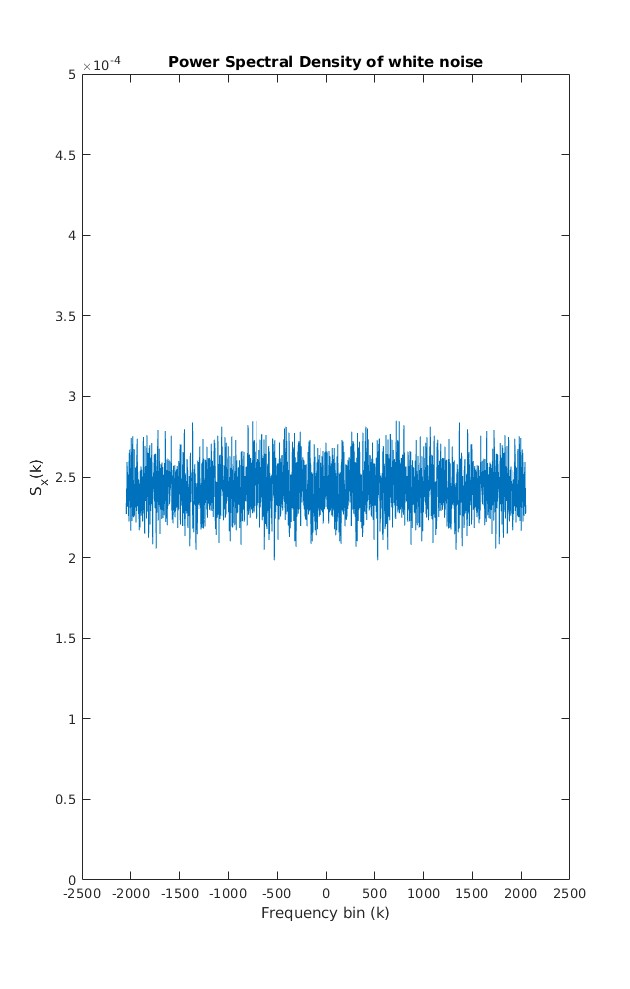
\includegraphics[width=0.5\linewidth]{Images/white_noise_spectral.jpg}
    \captionof{figure}{Power Spectral Density of White Noise}
    \label{fig:white-noise-density}
\end{center}

\item Figure \ref{fig:white-noise-autocorrelation} shows the autocorrelation for
Gaussian white noise with $N=10^5$ samples. At $\tau = 0$, the autocorrelation
function $R_x$ evaluates:
\begin{equation*}
    R_x(0) = E[x_n^2] = \sigma^2 = 1
\end{equation*}
where $\sigma$ is the standard deviation of the Gaussian distribution from which
the noise is sampled, and has been set to 1.

We see the autocorrelation function is center about 0 for $\tau > 0$, with the
variance increasing at high lag values. The mean of 0 indicates that $x_n$ and
$x_{n+k}$ are uncorrelated for all $n$ and $k \neq 0$.

At $\tau = k \delta t$ (where $\delta t$ is the sample timestep and $k$ is the
lag index), $R_x(k\delta t)$ is the sample mean of $N-k$ independent identically
distributed random variables, and therefore the variance decreases on the
order of $\sqrt{N-k}$. At high lag values $k$ is large, so the number of samples
$N-k$ is small. This explains why the variance increases at large lag values.

\begin{center}
    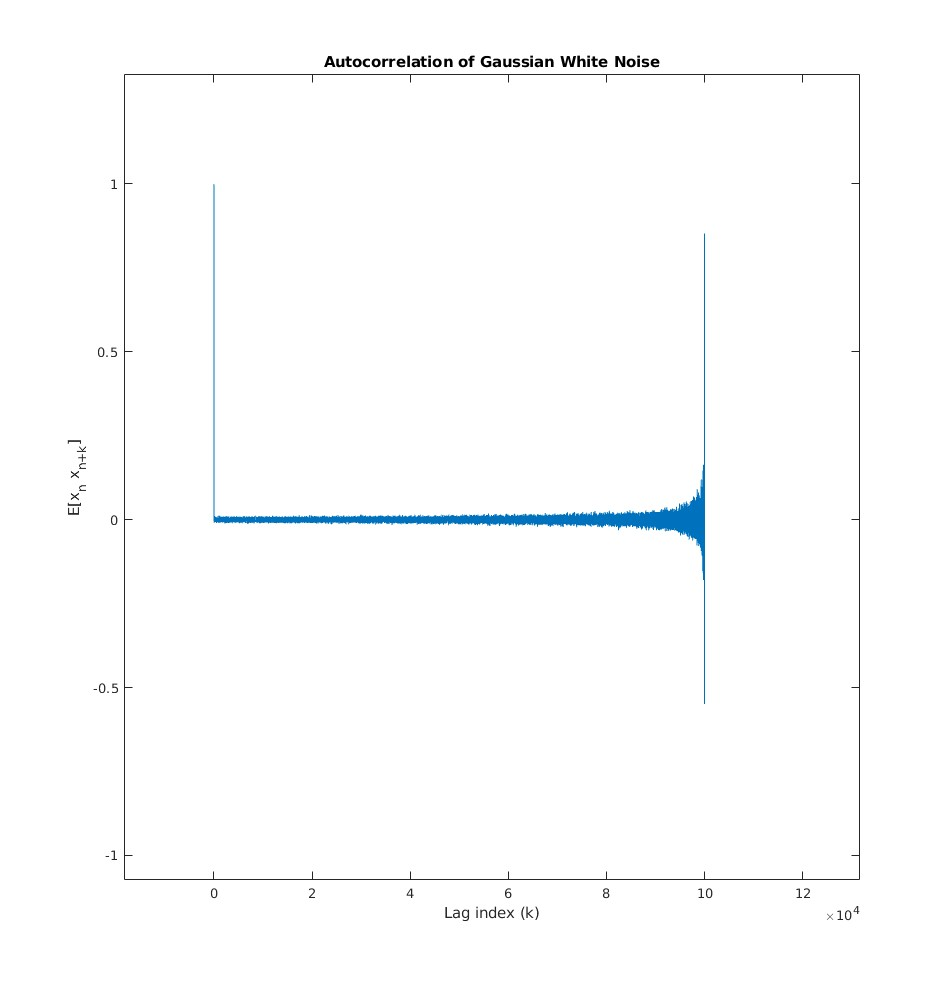
\includegraphics[width=0.5\linewidth]{Images/white_noise_autocorrelation.jpg}
    \captionof{figure}{Autocorrelation of White Noise}
    \label{fig:white-noise-autocorrelation}
\end{center}


\item The autocorrelation function for a cosine signal is a cosine function
of the same frequency with the phase shift removed.

Specifically, if $x(t) = cos (\omega t + \phi)$ where $\omega > 0$ is the angular
frequency and $\phi \in [0, 2\pi]$ is the phase shift, then the autocorrelation
function is given by:
\begin{equation}
    R_x(\tau) = 1/2 \cos(\omega \tau)
    \label{eq:autocorrelation-cos}
\end{equation}

A proof of this fact is provided in the appendix.
Figure \ref{eq:autocor-cosine} plots the numerically-computed autocorrelation
function, which closely coincides with equation (\ref{eq:autocorrelation-cos}).
The discrepancies can be attributed to the fact that the integral is numerically
approximated via a Riemann sum.


\begin{center}
    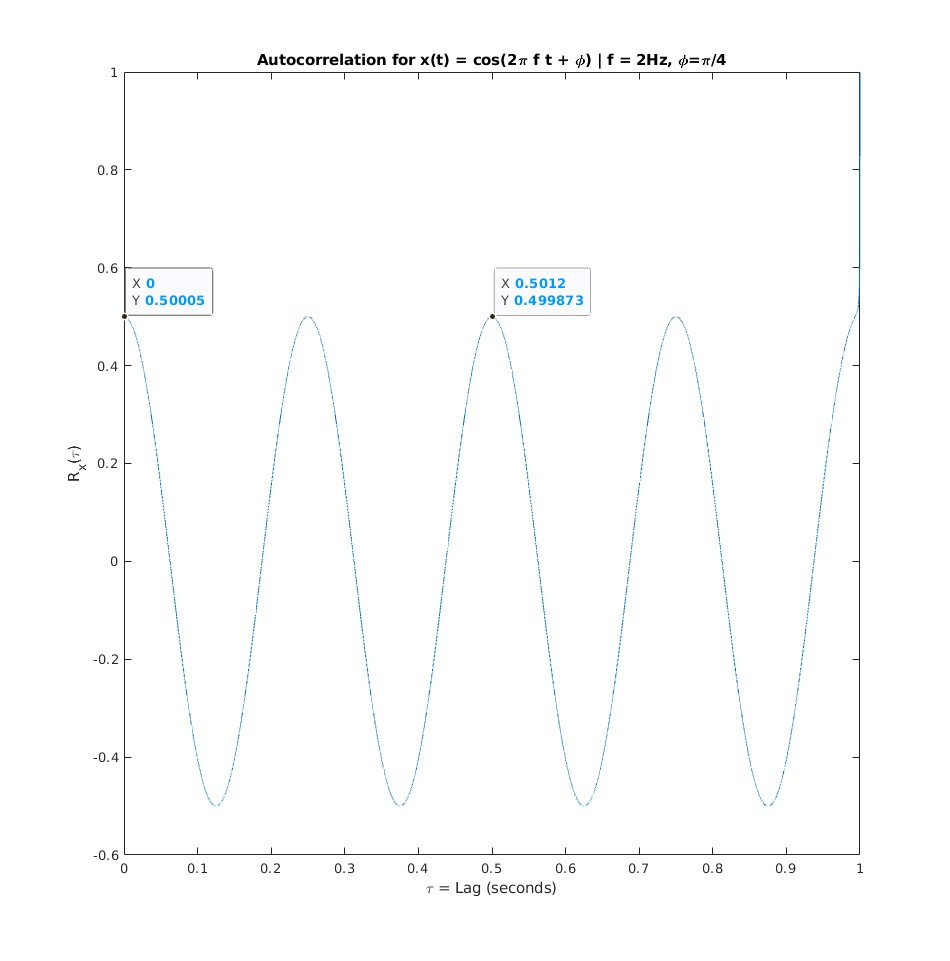
\includegraphics[width=0.5\linewidth]{Images/cosine_autocorrelation.jpg}
    \captionof{figure}{Autocorrelation of cosine function}
    \label{fig:cosine-autocor}
\end{center}


\end{enumerate}

\section{Problem 2}

Subsection \ref{sect:problem} provides a mathematical formulation
that will be referenced in answers in subsection \ref{sect:questions}.

\subsection{Problem Formulation}
\label{sect:problem}

Suppose a sequence $(\omega_i, H_i)\in (\R^N \times \C^N)$ of $N$ pairs
represents the measured angular frequency $\omega_i$ and frequency response $H_i$
of a system.

We assume these pairs arise from a rational function which we will estimate
with the complex-valued function $\hat{H}_m: \C \to \C$, given by:
\begin{equation}
    \hat{H}_m(s) = \frac{\sum_{\ell=0}^{L} a_\ell s^\ell}{1 + \sum_{k=1}^{K} b_k s^k}.
    \label{eq:tf-estimate1}
\end{equation}
where $L\geq0$ and $K>0$ are integers representing the number of zeros and poles, 
respectively.

The subscript $m$ indicates the dependence on the $M=(L+1)+K$-dimensional
model parameter $m\in\R^N$, consisting of the stack of polynomial coefficient
vectors $a\in\R^{L+1}$ and $b\in\R^K$. That is,
\begin{equation*}
    m = \mat{a \\ b} = \mat{a_0 \\ a_1 \\ \vdots \\ a_L \\ b_1 \\ \vdots \\ b_K}.
\end{equation*}
Note: we use matrix block notation here, as well as in subsequent equations.

We prefer to think of $\hat{H}_m$ as a vectorized function from $\C^N \to \C^N$
over the $N$ data points. Noting that the numerator and denominator
 are linear with respect to the model parameters, we rewrite
 (\ref{eq:tf-estimate1}) as
\begin{equation*}
    \hat{H}_m(s) = \frac{Sa}{1 + Tb}
\end{equation*}
where $S\in\C^{N\times L+1}$ and $T\in\C^{N \times K}$ are complex matrices,
dependent on the polynomial evaluations of the input $s=j [\omega_i]$
\begin{align*}
    S = \mat{1_{N\times 1} & s & \cdots & s^L} \\
    T = \mat{ s & s^2 & \cdots & s^K}
\end{align*}
To be clear, $s^i$ denotes the element-wise exponent of vector $s$.

To decide which of the rational functions approximates our given data best,
we need a error metric which defines quality of fit. The error function
$f: \R^M \to \R$, given by
\begin{equation*}
    f(m) := \sum_{i=1}^{N} |H_i - \hat{H}_m(s_i)|^2,
\end{equation*}
is nonlinear in terms of the model parameters so we multiply each error
term $H_i - \hat{H}_m(s_i)$ by $1 + T_i b$. Writing $T_i$ and $S_i$ to denote
the $i$th row of matrices $T$ and $S$, the modified error function
$g: \R^M \to \R$ can be writen in terms of matrix operations:
\begin{align*}
    g(m) &= \sum_{i=1}^{N} |H_i(1 + T_i b) - S_i a |^2 \\
        &= \sum_{i=1}^{N} |H_i - (S_i a - H_i T_i b)|^2 \\
        &= \sum_{i=1}^{N} \biggl|H_i - \mat{S_i &  -H_i T_i} \mat{a \\ b}\biggr|^2 \\
        &= \normtwo{h - Gm}^2.
\end{align*}
where $h = [H_i]^T \in \C^N$ is the vector of frequency responses, and the matrix
$G \in C^{N \times L + K + 1}$ is given by:
\begin{equation}
    G = \mat{
        S_1 & - H_1 T_1 \\
        S_2 & - H_2 T_2 \\
        \vdots & \vdots \\
        S_N & - H_N T_N
    } = \mat{S & \text{diag}(h) T}
    \label{eq:G-matrix}
\end{equation}


To enforce that the model parameters
$m$ are real, we convert solve the real-valued least squares (LS) problem
\begin{equation}
    \mat{\Re (G) \\ \Im(G)} m = \mat{\Re(h) \\ \Im(h)}
    \label{eq:least-squares}
\end{equation}
where $\Re$ and $\Im$ take the real and imaginary components, respectively, of $G$
and $h$.


\subsection{Questions}
\label{sect:questions}

\begin{enumerate}[label=\roman*)]
\item We implement the rational function fitting based on the least squares
formulation, as discussed in lecture.
The code is provided in the appendix and parallels the mathematical formulation
of the previous section.

A plot of the fit with $L=2$, $K=2$ is shown in figure \ref{fig:ls-no-noise}. 
The model vector is found to be:
\begin{equation*}
    m = \mat {a_0 \\ a_1 \\ a_2 \\ b_1 \\ b_2} \approx \mat{
        0.125 \\
        0.25 \\
        0 \\
        0.1 \\
        0.0025
    }
\end{equation*}
so that the estimated transfer function $\hat{H}_m(s)$ is given by:
\begin{equation*}
    \hat{H}_m(s) = \frac{0.125 + 0.25 s}{1 + 0.1s + 0.0025s^2}
        = \frac{(s - z_1)(s - z_2)}{(s - p_1)(s - p_2)}
\end{equation*}
where the poles are zeros are
\begin{equation*}
    z_{1} = -0.5 \qquad z_2 = 9\cdot 10^{13} \qquad
    p_{1,2} = -20 \pm j 0.1
\end{equation*}
The location of $z_2$ far outside the frequency range suggests that only
a first degree polynomial is necessary to represent the numerator.

\begin{center}
    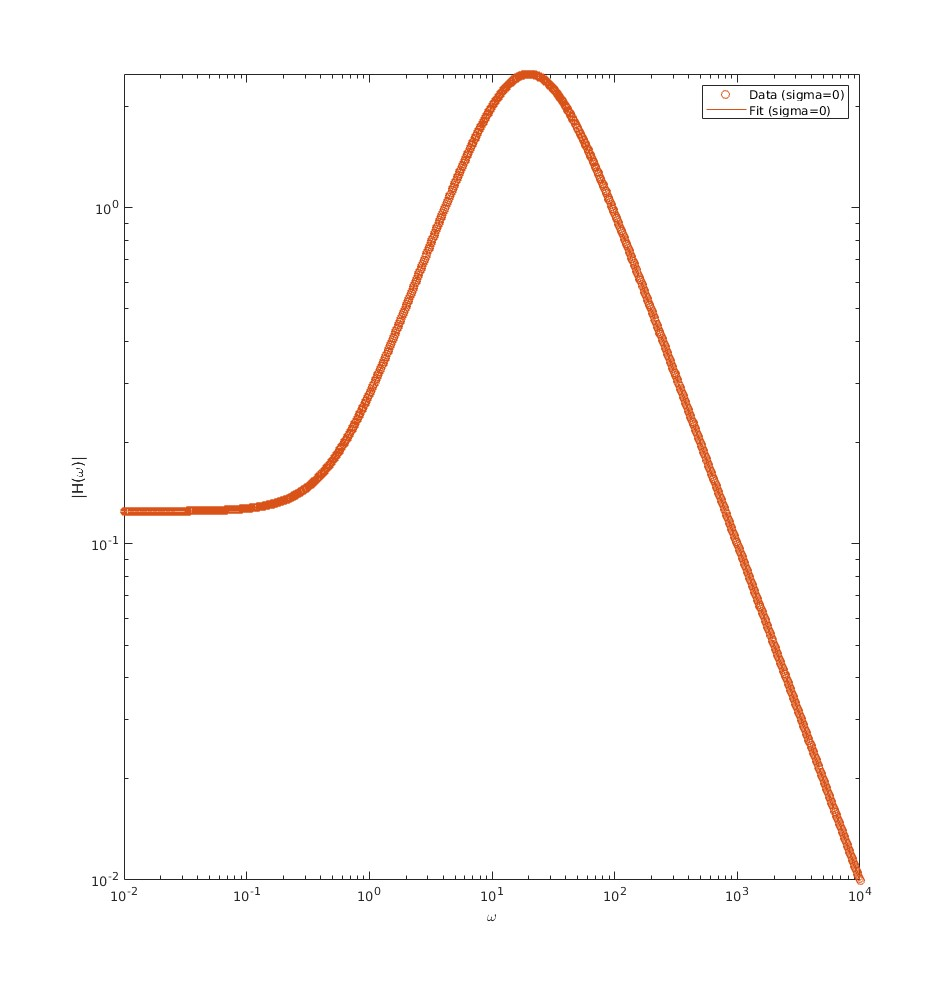
\includegraphics[width=0.8\linewidth]{Images/ls_fit_no_noise.jpg}
    \captionof{figure}{Least squares fit ($L$=2, $K$=2) with no noise added}
    \label{fig:ls-no-noise}
\end{center}

Figure \ref{fig:ls-no-noise-zoomed} zooms in to show that the fit, indeed coincides
closely with the given data.

\begin{center}
    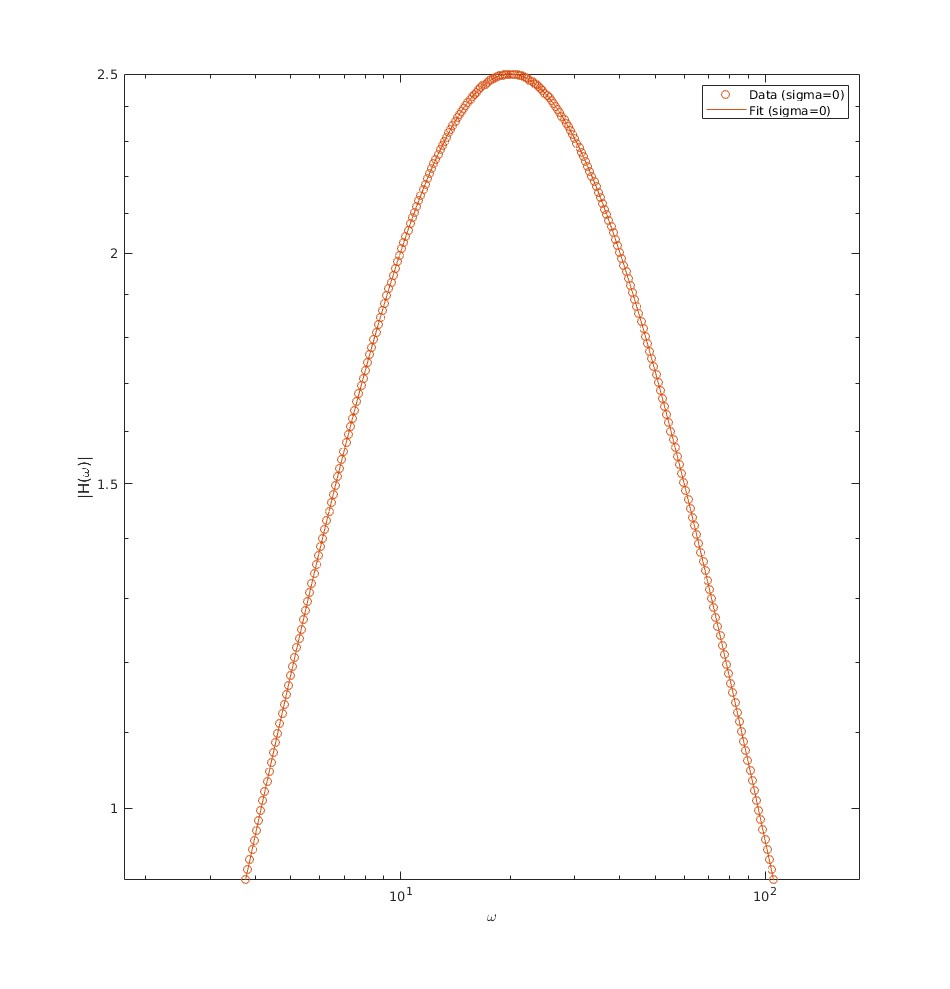
\includegraphics[width=0.8\linewidth]{Images/ls_fit_no_noise_zoom.jpg}
    \captionof{figure}{Least squares fit ($L$=2, $K$=2) with no noise added (zoomed)}
    \label{fig:ls-no-noise-zoomed}
\end{center}


\item A fit for the model with $L=1$ and $K=1$ is shown in Figure
\ref{fig:ls-no-noise-1-deg}. Unlike the previous plot, this does not fit
the data well. This suggests that the original function has at least two poles.
When adding additional poles ($K>2$), the plot looks very similar to the one
above for $K=2$, which suggests that the original function has exactly two distinct
poles.


\begin{center}
    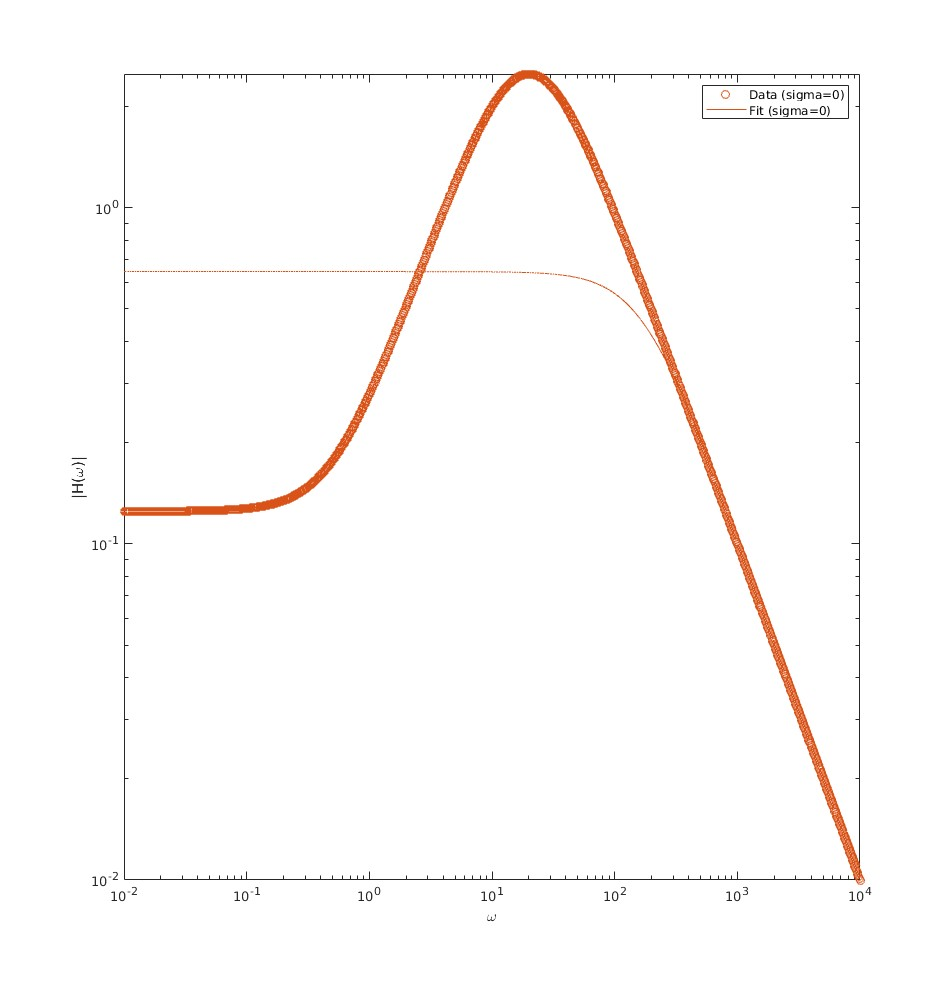
\includegraphics[width=0.8\linewidth]{Images/ls_no_noise_deg_1.jpg}
    \captionof{figure}{Least squares fit with no noise added ($L=K=1$)}
    \label{fig:ls-no-noise-1-deg}
\end{center}



\item Plots for the function fit with the prescribed noise values added
are shown in Figure \ref{fig:ls-noise}.  A zoomed in view is shown in figure
\ref{fig:ls-noise-zoomed}.

\begin{center}
    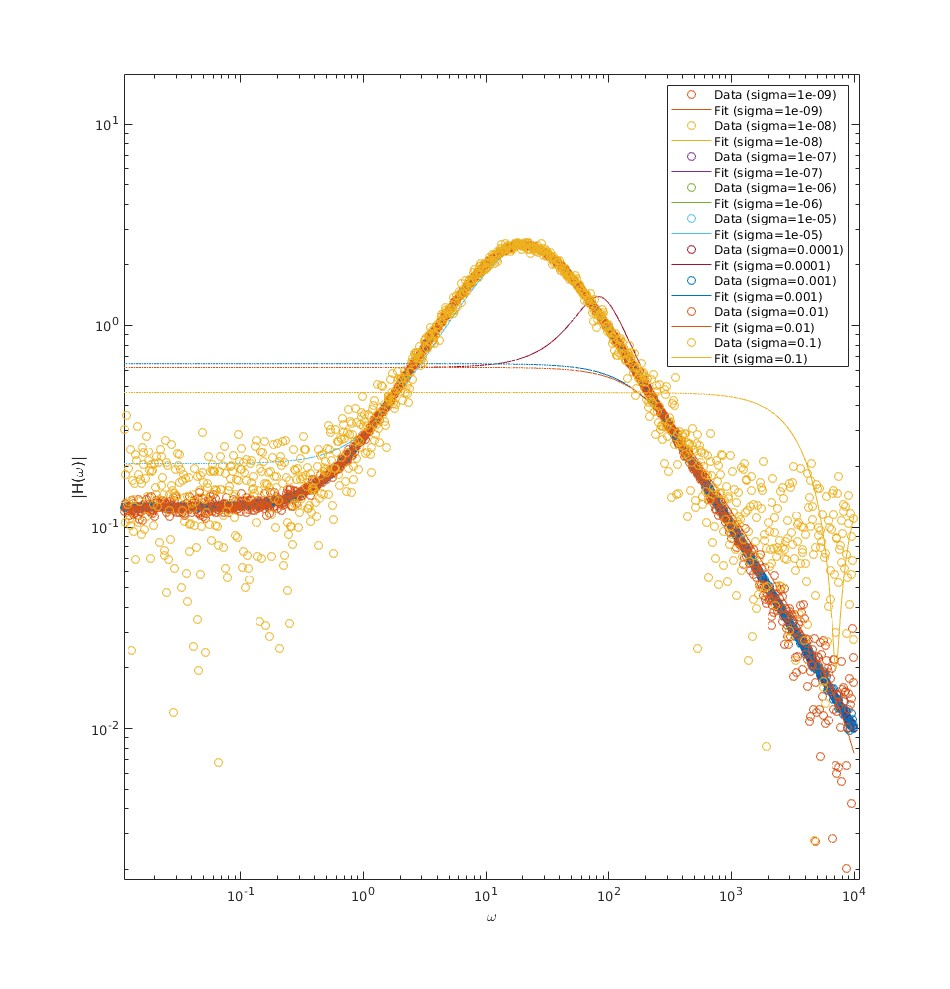
\includegraphics[width=0.8\linewidth]{Images/ls_noise.jpg}
    \captionof{figure}{Least squares fit with noise added ($L=K=2$)}
    \label{fig:ls-noise}
\end{center}

\begin{center}
    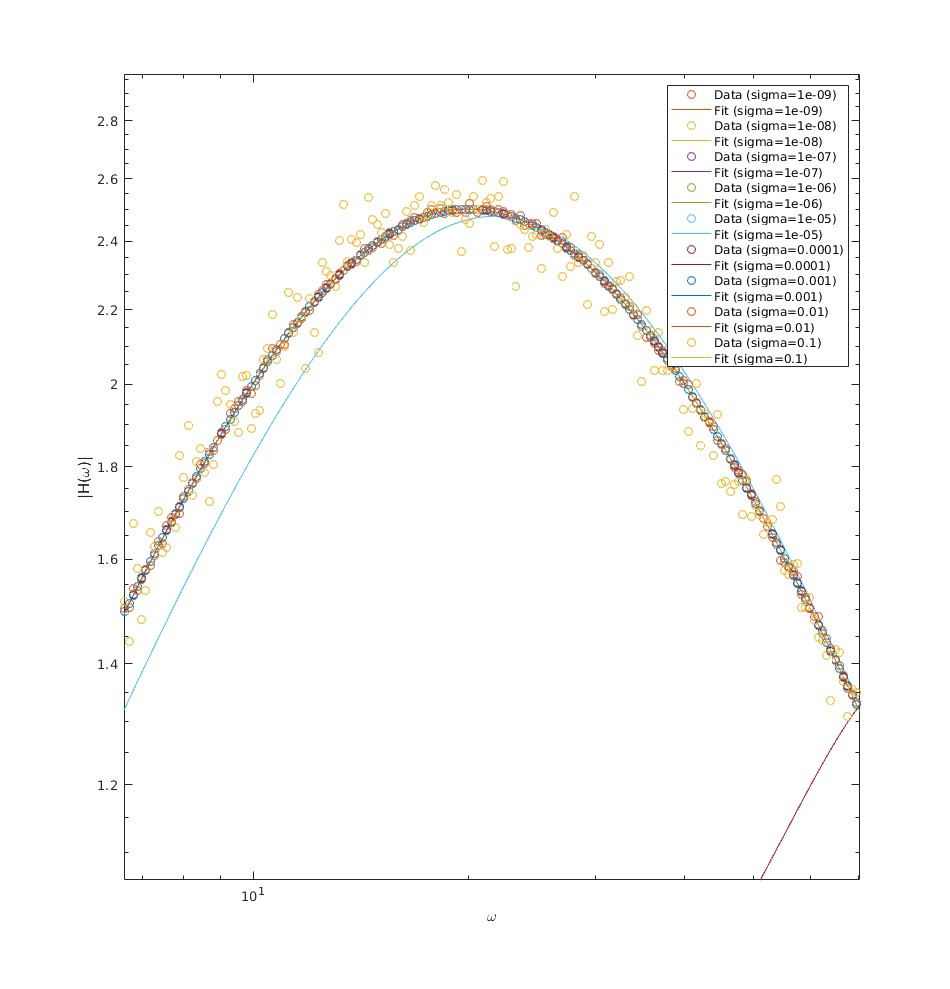
\includegraphics[width=0.8\linewidth]{Images/ls_noise_zoom.jpg}
    \captionof{figure}{Least squares fit with noise added ($L=K=2$)}
    \label{fig:ls-noise-zoomed}
\end{center}

\item From Figures \ref{fig:ls-noise} and \ref{fig:ls-noise-zoomed},
we see that the fit for $\sigma = 1e-5$ begins to diverge visibly from
true transfer function. Each $\sigma > 1e-5$ diverges increasingly more
dramatically.

Perhaps a more interesting question than "when does the fit break down"
is "why does the fit break down"? The condition number $\kappa(G)$ of the
matrix $G$ provides some insight. Consider the following perturbed version
of the least squares problem:
\begin{equation*}
    G(m + \delta m) = h + \delta h
\end{equation*}
where $\delta h\in\C^N$ is the perturbation in the input to the LS problem and
$\delta m \in \R^N$ is the resulting perturbation in our model. (In this case
the matrix $G$ is a function of $h$ per equation(\ref{eq:G-matrix}), but we will
neglect that for conceptual clarity. This simplification is justified later:
see Figure \ref{fig:cond-vs-noise}.)

The condition number provides a bound on the ratio between the relative model error
$\norm{\delta m} / \norm{m}$ and the relative input error
$\norm{\delta h} / \norm{h}$. That is,
\begin{equation*}
    \frac{\frac{\norm{\delta m}}{\norm{m}}}{\frac{\norm{\delta h}}{\norm{h}}}
        \leq \kappa(G)
\end{equation*}

When $\kappa(G)$ is large, the least squares problem is said to be
{\it ill-conditioned}.

A geometric interpretation is that the input $h + \delta h$
exists in some ball $\mathcal{H}$ of radius $\delta h$ center around $h$. Solution of the least square
problem maps this region to ball $\mathcal{M}$ centered at $m$ with radius
$\delta m$.  The larger the condition number, the more this map from $\mathcal{H}$
to $\mathcal{M}$ is an expansion.

Figure \ref{fig:cond-vs-noise} shows that the condition number is on the
order of $1e7$ and varies only slightly as a function of the input noise.

\begin{center}
    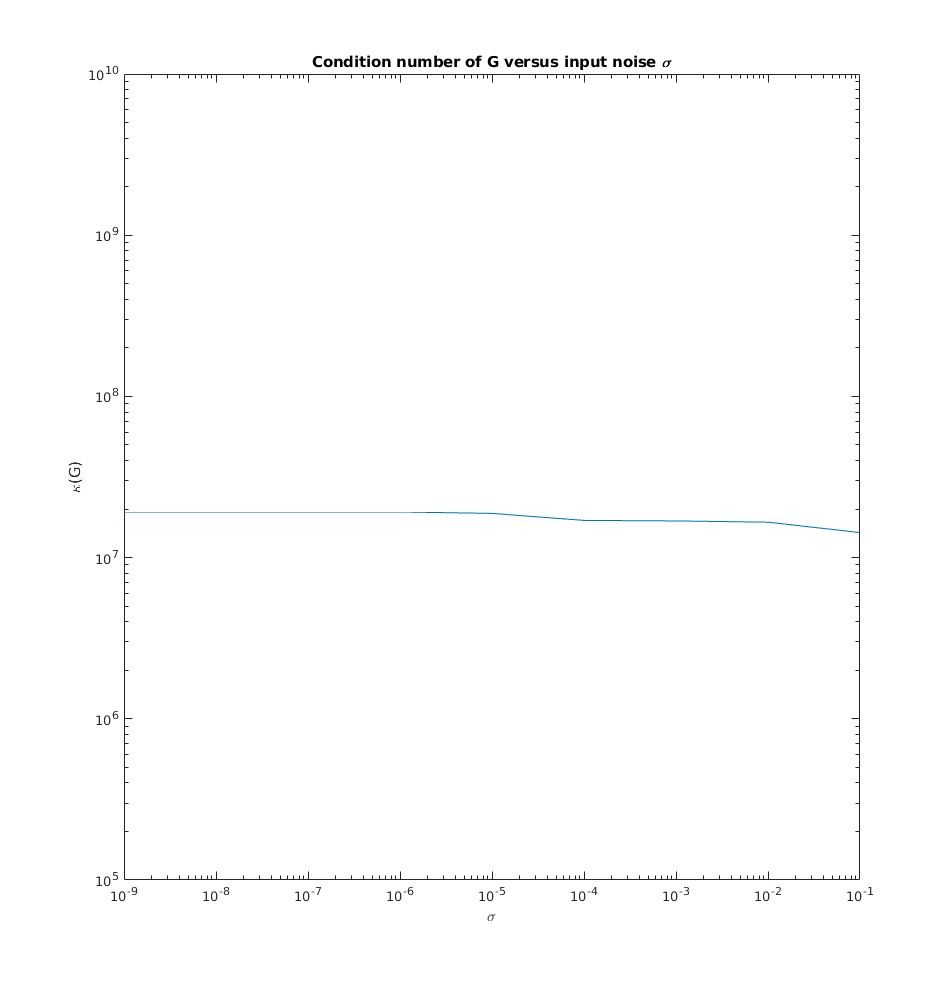
\includegraphics[width=0.6\linewidth]{Images/condition_number_vs_noise.jpg}
    \captionof{figure}{Condition number of $G$ as a function of $\sigma$}
    \label{fig:cond-vs-noise}
\end{center}

\def\code#1{\texttt{#1}}

We define
\begin{equation*}
    \alpha = \frac{\max_i \omega_i}{\min_i \omega_i}
\end{equation*}
to be the dynamic range. Then, the ratio between the minimum and maximum entries of $s^K$
(the $K$-th column of the matrix $T$) scales with $\alpha^K$. This suggests that
the condition number will also scale poorly with the number of poles $K$.
Indeed, figure \ref{fig:cond-vs-poles} shows that this to be the case.

\begin{center}
    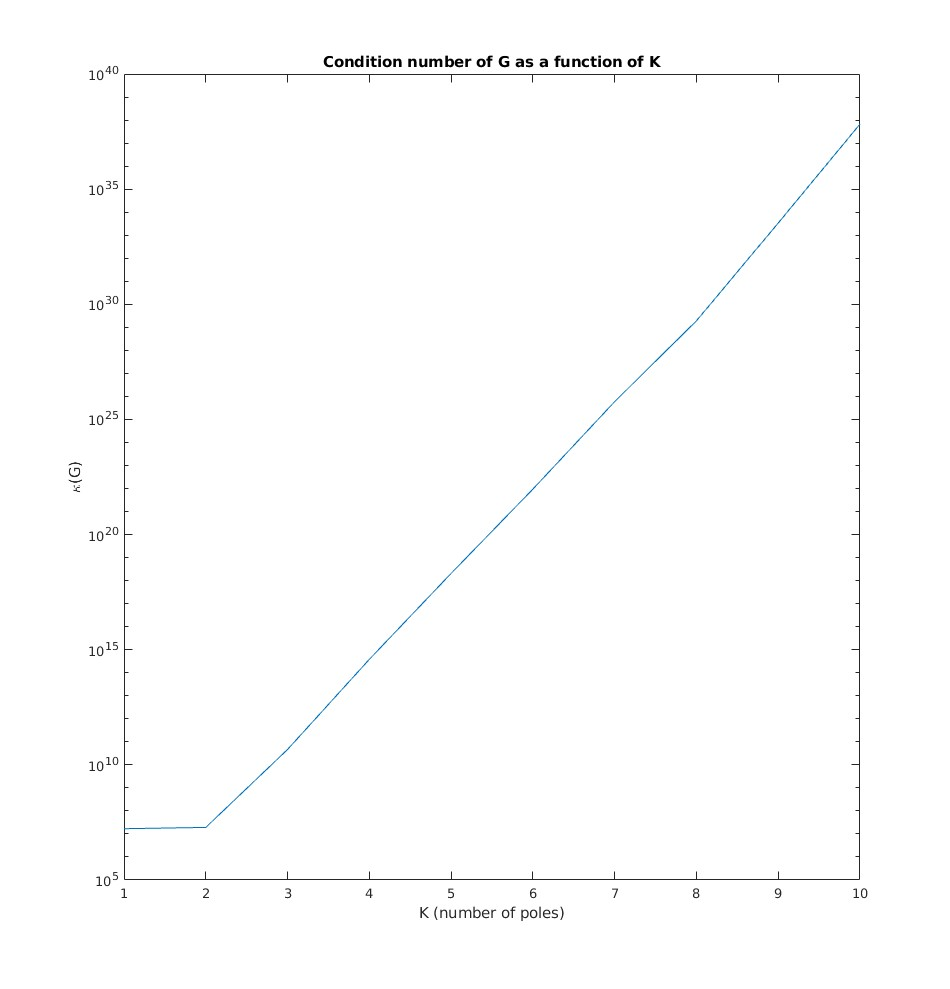
\includegraphics[width=0.8\linewidth]{Images/condition_number_vs_poles.jpg}
    \captionof{figure}{Condition number of $G$ as a function of the number of poles $K$}
    \label{fig:cond-vs-poles}
\end{center}

The moral of the story: if you want to reduce the sensitivity of model output
to input noise, you should formulate the problem in a well-conditioned manner.
\cite{rational} also notes this conditioning issue, and proposes an alternative
formulation which tackles the problem in a more robust way.
The RF toolkit MATLAB package provides a function called \code{rational} which
implements this alternative algorithm (or something similar).

We have performed the fit using \code{rational} and displayed the results
in Figures \ref{fig:rational-fit} and \ref{fig:rational-fit-zoom}.
Evidently, this alternative algorithm continues to track
the true solution even at high levels of noise.

\begin{center}
    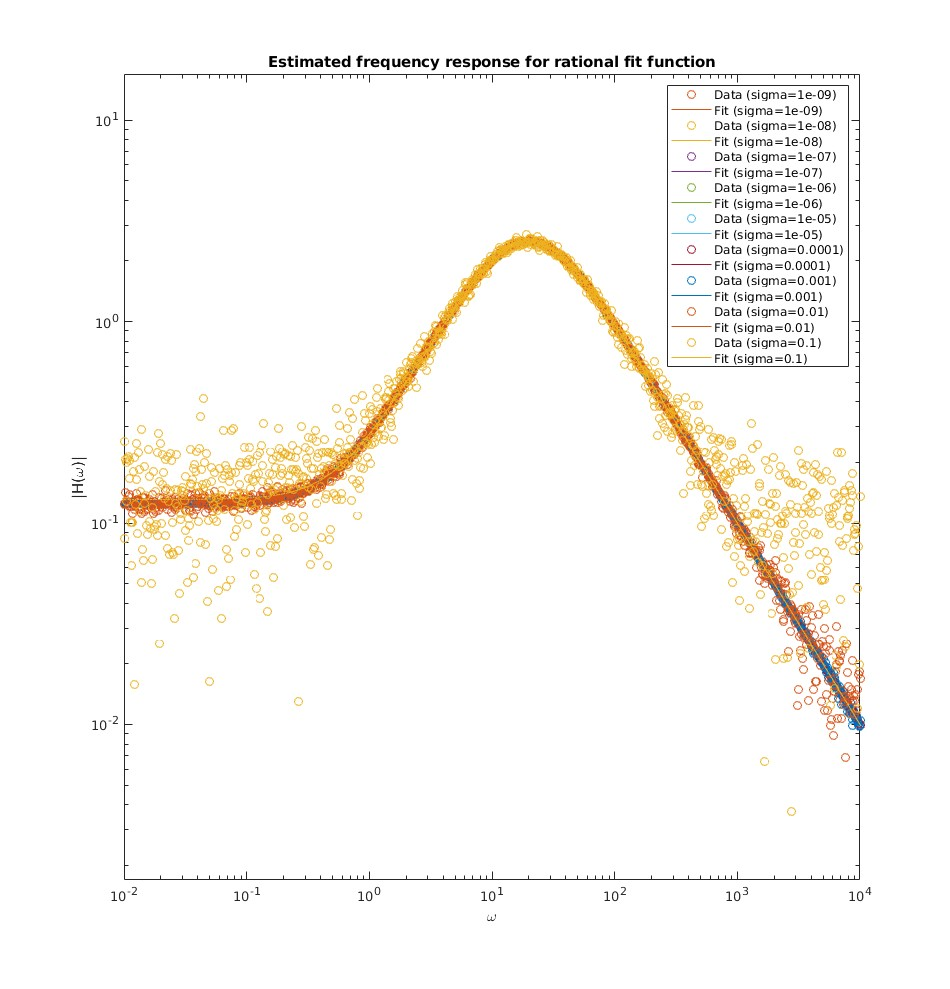
\includegraphics[width=0.8\linewidth]{Images/rational_fit.jpg}
    \captionof{figure}{Data points vs. \code{rational} fit for various values of $\sigma$}
    \label{fig:rational-fit}
\end{center}
\begin{center}
    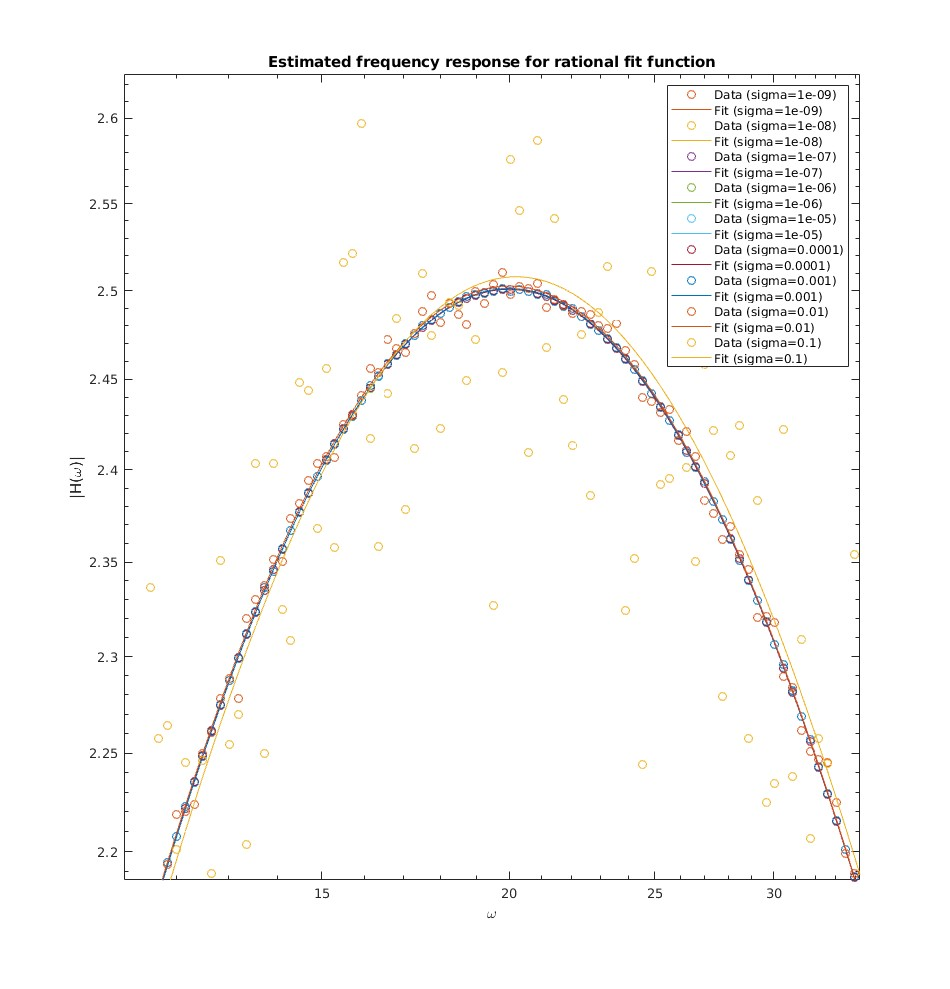
\includegraphics[width=0.8\linewidth]{Images/rational_fit_zoom.jpg}
    \captionof{figure}{Data points vs. \code{rational} fit for various values of $\sigma$ (Zoomed)}
    \label{fig:rational-fit-zoom}
\end{center}

\item $\chi^2$ and Pearson coefficients for both the LS and \code{rational}
fit are shown in figures \ref{fig:chi2}, \ref{fig:chi2-zoom}, and \ref{fig:pearson}.


\begin{center}
    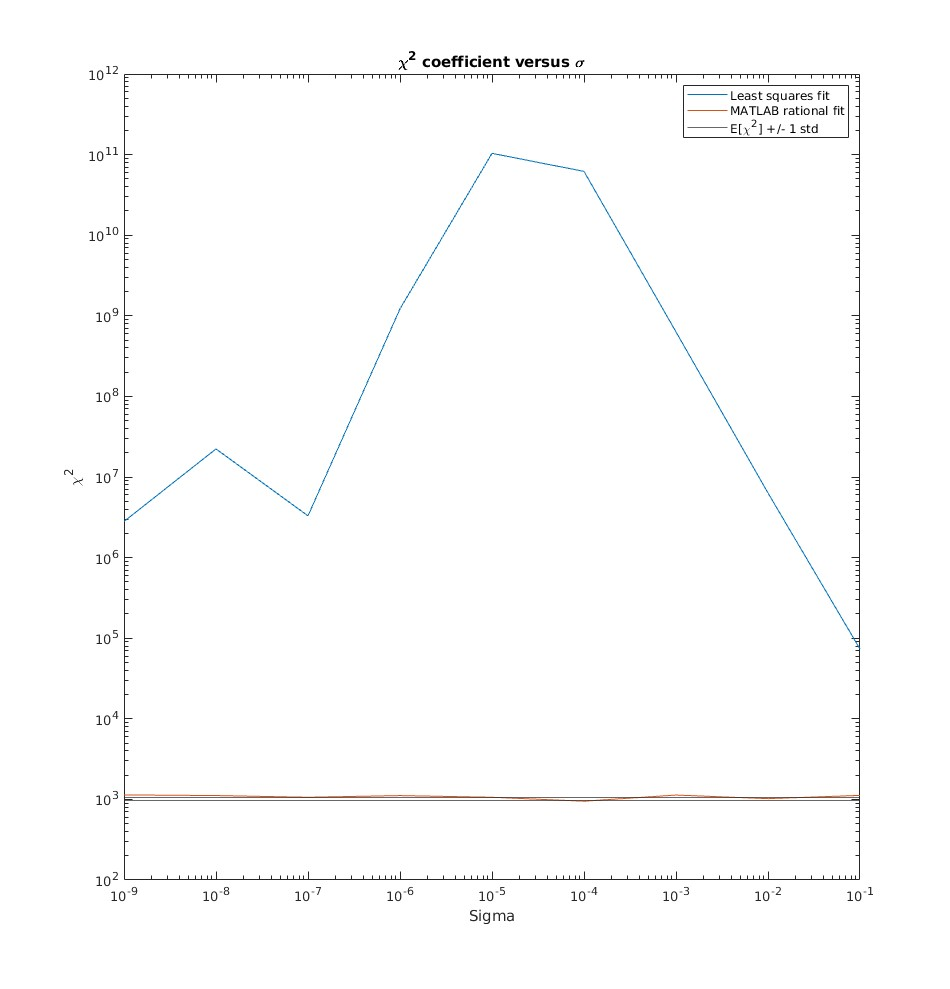
\includegraphics[width=0.8\linewidth]{Images/chi2_vs_sigma.jpg}
    \captionof{figure}{$\chi^2$ Goodness-of-fit Coefficient}
    \label{fig:chi2}
\end{center}
\begin{center}
    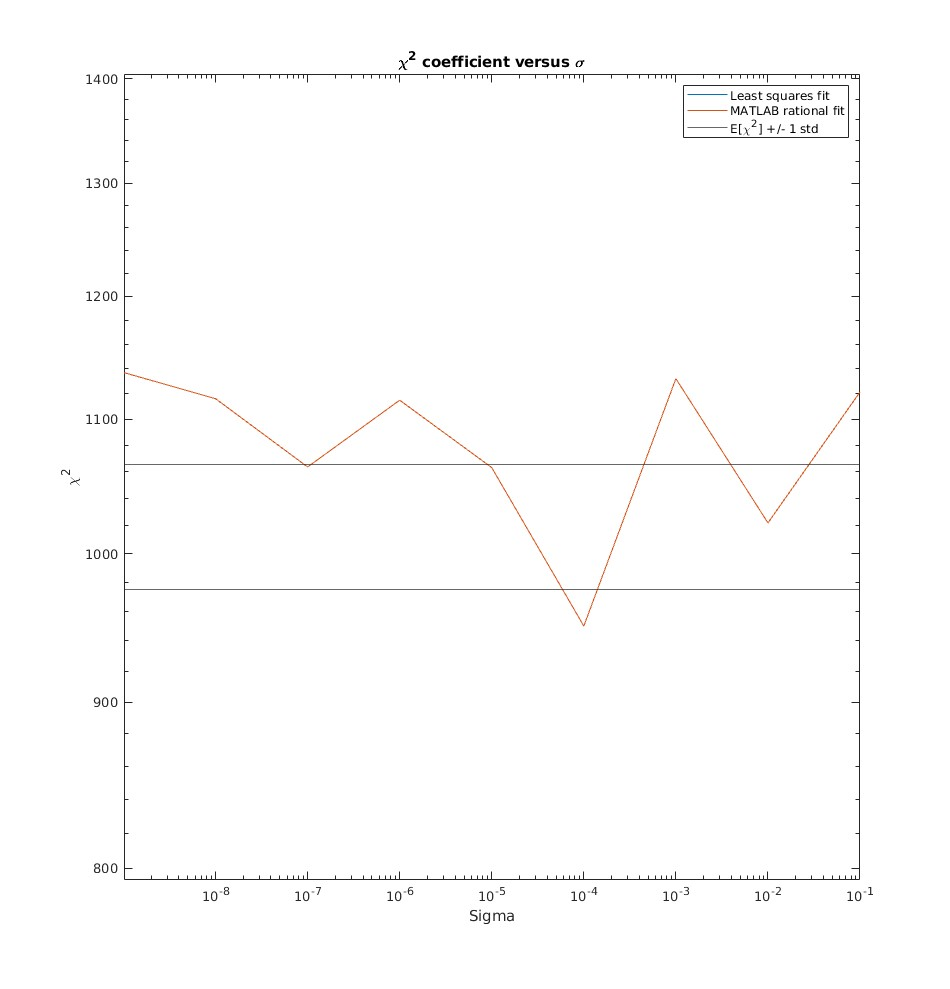
\includegraphics[width=0.8\linewidth]{Images/chi2_vs_sigma_zoom.jpg}
    \captionof{figure}{$\chi^2$ Goodness-of-fit Coefficient (Zoom)}
    \label{fig:chi2-zoom}
\end{center}
\begin{center}
    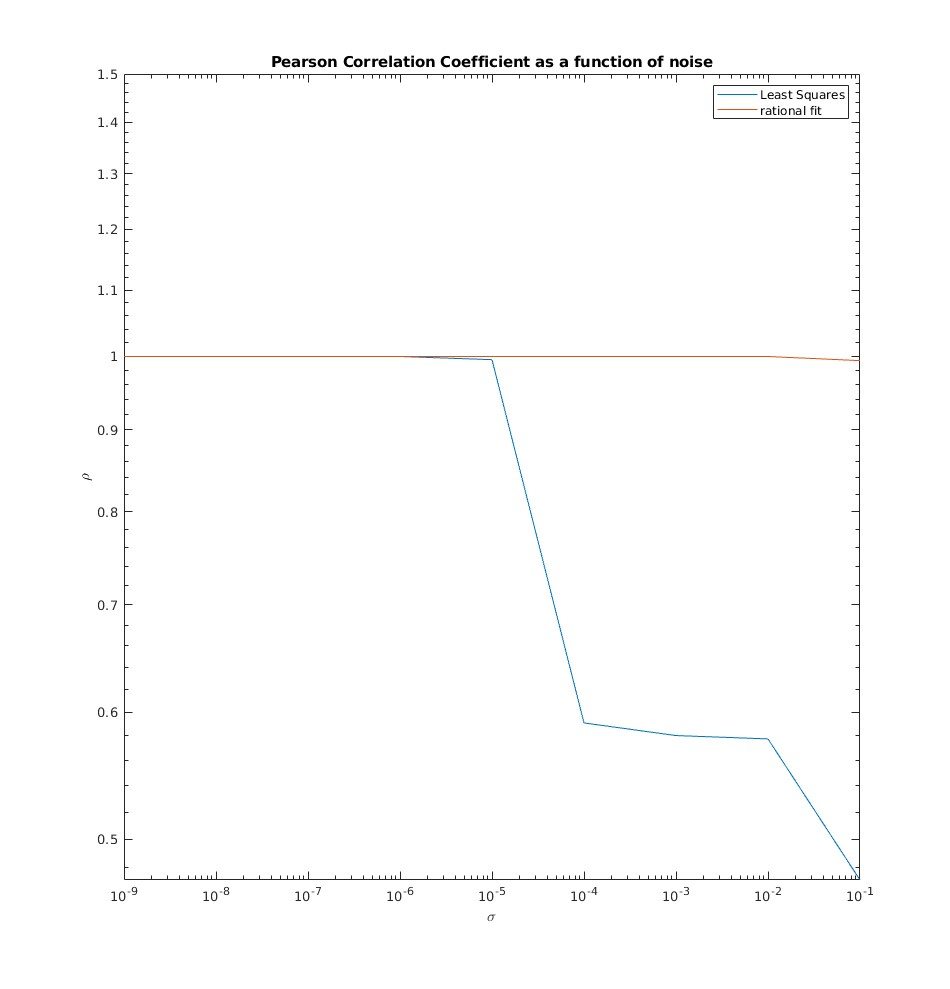
\includegraphics[width=0.8\linewidth]{Images/pearson_coef.jpg}
    \captionof{figure}{Pearson Correlation Coefficient (Zoom)}
    \label{fig:pearson}
\end{center}


\item Interpreted geometrically, the Pearson Correlation coefficient
provides a measure of the angle between vectors $h$ and $\hat{H}_m(s)$ in $\C^N$.
Consider the standard inner product on $\C^N$ given by:
\begin{equation*}
    \langle a, b \rangle = \sum_{i=1}^{N} a_i b_i^*
\end{equation*}

The Pearson coefficient therefore can be written
\begin{equation*}
    \rho = \frac{\langle h, \hat{H}_m(s) \rangle}{\normtwo{h} \normtwo{\hat{H}_m(s)}}
\end{equation*}
The analogy to $\R^N$ is that the angle $\theta$ between two vectors $x,y\in\R^N$
is given by:
\begin{equation*}
    \cos(\theta) = \frac{\langle x, y \rangle}{\normtwo{x} \normtwo{y}}
\end{equation*}

This perspective helps explain why the Pearson coefficient succeeds in identifying
the point at which the solution degenerates away from the true transfer function.
However, I would suggest that Pearson coefficient is actually somewhat misleading.
It obscures the numerical instability that occurs at all noise levels. 

I would argue that the $\chi^2$ coefficient is actually the more useful
coefficient in this case because it highlights issues with numerical stability.

For additional insight into the validity of the $\chi^2$ and Pearson
coefficients, we plot the distribution of the error vector $e \in \C^N$
given by $e = h + \delta h - \hat{H}_m(j \omega)$. Even when $\sigma = 1e-9$, 
the error in the LS estimates far exceeds the original perturbation.

Figure \ref{fig:error-dist-ls} shows a histogram of the magnitude $|e|$ is
shown for the LS solution.
while figure \ref{fig:error-dist-rational} shows the same plot for
the \code{rational} solver. Note the
logarithmic scale of the LS solution plot. The red line corresponds to the
distribution of the magnitude of the input pertubation $|\delta h|$, which is drawn
from the one-sided Gaussian with PDF $p_{|\delta h|}$ given by:
\begin{equation*}
    p_{|\delta h|}(d) = \biggl\{
        \begin{array}{ll}
            2 \cdot \frac{1}{\sqrt{2\pi} \sigma} e^{d^2 / 2\sigma^2}
                &\qquad \text{ if } d \geq 0 \\
            0 & \qquad \text{otherwise}
        \end{array}
    \biggr.
\end{equation*}

\begin{center}
    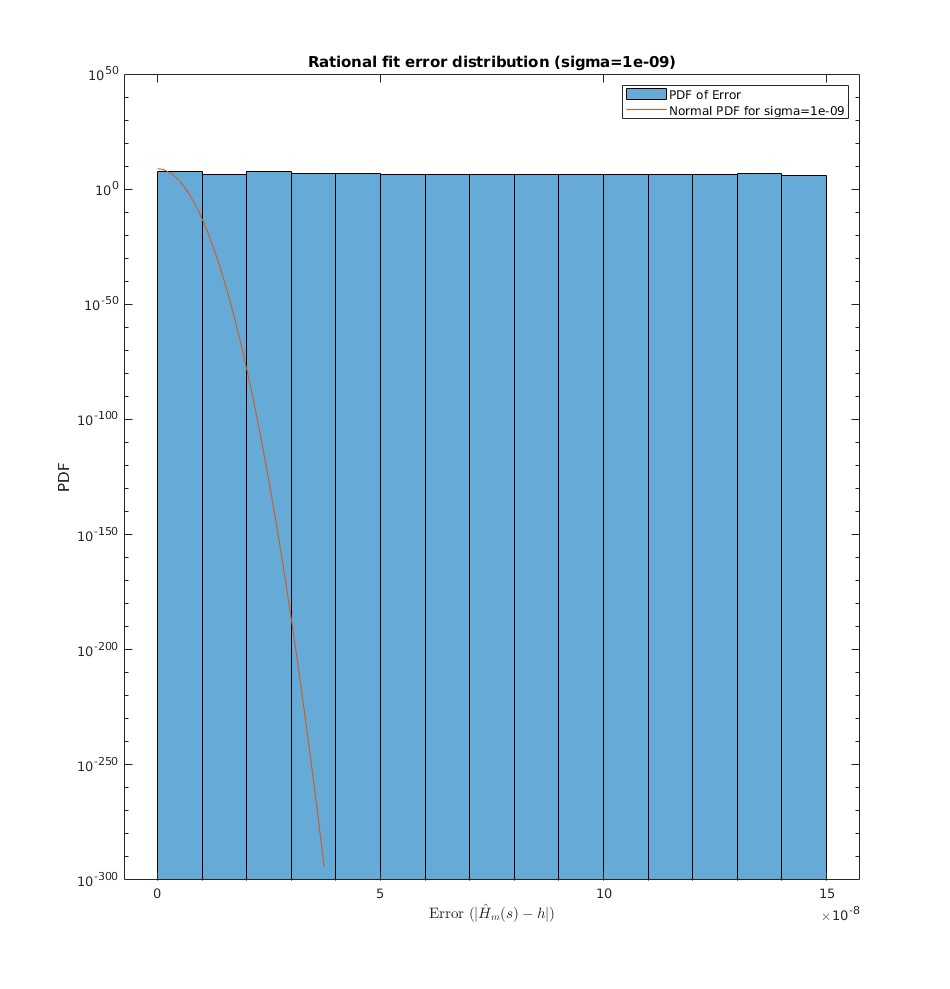
\includegraphics[width=0.8\linewidth]{Images/error_dist_ls.jpg}
    \captionof{figure}{Error distribution for LS solution}
    \label{fig:error-dist-ls}
\end{center}

\begin{center}
    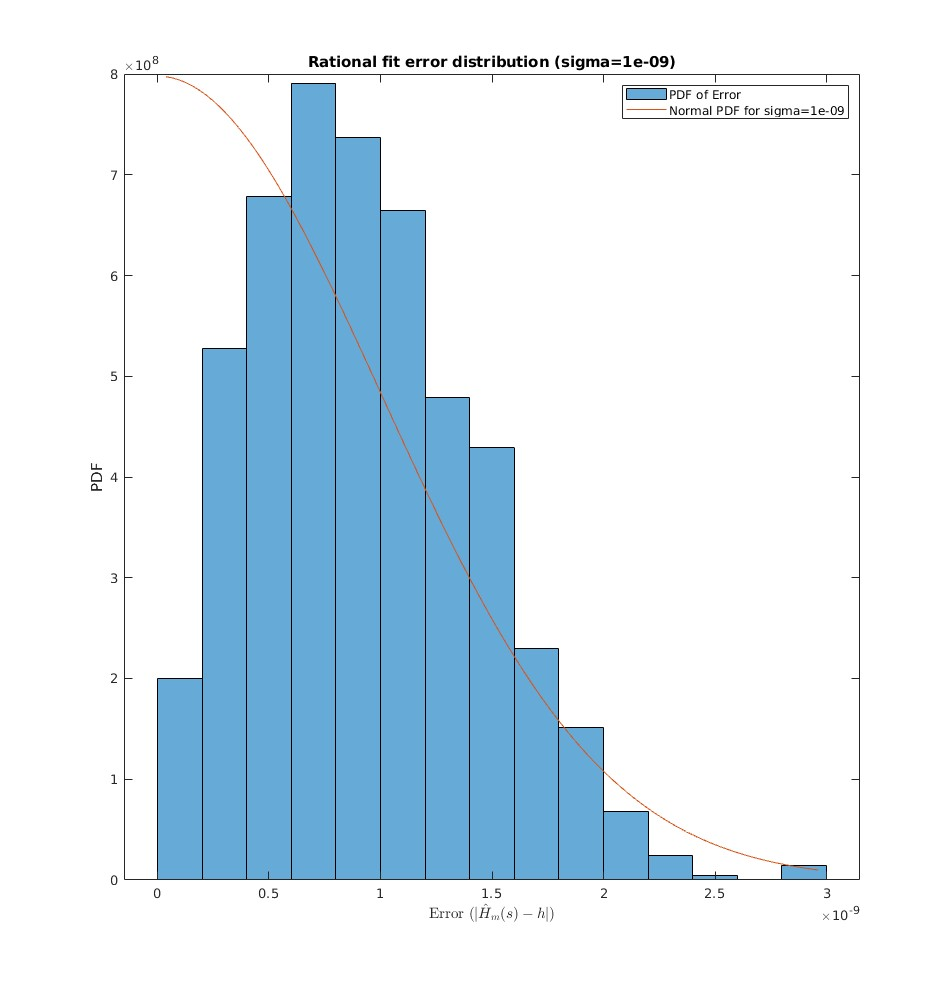
\includegraphics[width=0.8\linewidth]{Images/error_dist_rational.jpg}
    \captionof{figure}{Error distribution for \code{rational} solution}
    \label{fig:error-dist-rational}
\end{center}

Plots for larger $\sigma$ are similar qualitatively. While the solution does
not degenerate until around $\sigma \geq 1e-5$, the ill-conditioning of the LS
problem means that the error $|e|$ in our estimates represents a significant
amplification of the input noise $\delta h$, which seems undesirable in all scenarios.

Interestingly, the error distribution for the \code{rational} solution is also
no longer Gaussian, and appears to be closer a $\chi^2$ or Poisson distribution
in shape.
However, in order of magnitude, the estimate error is significantly closer
to the distribution of $|\delta h|$.
This explains why the computed $\chi^2$ coefficients plotted in figure
\ref{fig:chi2-zoom} are quite close to the expected range. 

The crux of the issue here seems not to be the selection of goodness-of-fit coefficient, but
rather the algorithm which generated the fit in the first place! In light of this, outside of
pedagogy, is there any scenario where the LS solution would be prefered to the one provided
by \code{rational}?



% Remaining Todo:
% ~~iii) plot bode of all sigmas and zoomed~~
% iv) ~~Discussion of breakdown --~~
% ~~The problem is ill-conditioned~~
% ~~Moral of the story: if you want to fit high degree polynomial over a large range
% of frequencies without introducing numerical inaccuracy, you should use
% alternative algorithms to the least squares formulation presented in lecture.
% Condition number as bounding the error vector $\delta h$~~
% Plot: Condition number of matrix vs sigma
% ~~Using higher order polynomials or larger frequency ranges exacerbate the issue~~
% Plot: Condition number of matrix vs degree of polynomial
% ~~Via a different problem formulation and algorithmic solution, this issue can
% be avoided: ~~
% v) Plots of pearson and chi2 coefficients
% vi) Discussion of Pearson Correlation coefficient
% effectively measures the angle between
% the vector H and the estimated \hat{H} -- this is good at detecting when
% the vector has significantly diverged from measured data, but obscures the
% fact that the fit is amplifying the measurement noise. 
% Issues with numerical stability are evident at all noise values, as shown
% by the \chi2 figure. A look at the error distrubtion shows the distribution
% is not at all normally distributed
% interestingly the error distribution is no longer a zero-mean (1-sided) Gaussian,
% but looks more chi2 or poisson.








\end{enumerate}

\section{Appendix}
\subsection{Fact 1}

Suppose $x(t) = \cos(\omega t + \phi)$ for some numbers $\omega$ and $\phi$.
We want to show that $R_x(\tau) = 1/2 \cos(\omega \tau)$.

Since $x$ is periodic with period $T=2\pi/\omega$, the autocorrelation function
can be found by integrating over a single period:
\begin{equation}
    R_x(\tau) = E[x_t x_{t+\tau}^*] = \frac{1}{T} \int_{0}^{T}
        cos(\omega t + \phi) cos(\omega(t + \tau) + \phi) dt.
        \label{eq:autocor-cosine}
\end{equation}

Using the product-to-sum identity
\begin{equation*}
    \cos(a) \cos(b) = \frac{1}{2} (\cos(a+b) + \cos(a - b)),
\end{equation*}
with $b = \omega t + \phi$ and $a=\omega(t + \tau) + \phi$, equation
\ref{eq:autocor-cosine} simplifies to:
\begin{align*}
    R_x(\tau) &= \frac{1}{2T} \int_{0}^{T} \cos(a+b) + \cos(a - b) dt \\
        &= \frac{1}{2} \biggl(\frac{1}{T} \int_{0}^{T} \cos(2\omega t + \alpha) dt
            + \cos (\omega \tau) \int_{0}^{T} \frac{1}{T} dt\biggr) \\
        &= \frac{1}{2} \cos(\omega \tau)
\end{align*}
where $\alpha = \omega \tau + 2 \phi$. The first integral integrates over two
periods of a cosine function with frequency $2\omega$ and therefore sums to 0,
while the second integral is constant with respect to $t$.

\subsection{MATLAB implementation for Problem 1}
\begin{lstlisting}
N = 1e5;
n = randn(N, 1);

function S = periodogram(x, N, overlap, window_func)
    L = size(x, 1);  % Total number of samples
    P = floor((L-overlap) / (N - overlap));

    w = window_func(N);
    wss = sum(w.^2)/N;
    S = zeros(N,1);
    index = 1:N;
    for i=1:P
        S = S + abs(fft(x(index) .* w)).^2;
        index = index + (N - overlap);
    end
    S = fftshift(S) / (M * N^2 * wss);
end

function Rx = autocorrelation(x)
    L = size(x, 1);
    Rx = zeros(size(x));
    disp(L)
    for n=1:L
        Rx(n) = x(1:L-n+1)' * x(n:L) / (L-n);
    end
end

N_sample = 4096;
overlap = N_sample/4;
S_f = periodogram(n, N_sample, overlap, @blackman);


figure()
plot(n)
xlabel("Index (n)")
ylabel("x(n)")
title("White Gaussian Noise (\sigma=1)")

f_fft = (0:N-1) - N/2;
S_f_fft = fftshift(abs(fft(n).^2)/N^2);

f_periodogram = (0:N_sample-1) - N_sample/2;
N_sample = 4096;
overlap = N_sample/4;
S_f_periodogram = periodogram(n, N_sample, overlap, @blackman);

figure()
plot(f_periodogram, S_f_periodogram)
ylim([0, 5e-4])
xlabel("Frequency bin (k)")
ylabel("S_x(k)")
title("Power Spectral Density of white noise")

fprintf("Power from original: %g\n", 1/N * n' * n);
fprintf("Power from spectrum: %g\n", sum(S_f_fft));
fprintf("Power from periodogram: %g\n", sum(S_f_periodogram));

figure()
Rx = autocorrelation(n);
plot(Rx);
title("Autocorrelation of Gaussian White Noise")
xlabel("Lag index (k)")
ylabel("E[x_n x_{n+k}]")

%% Autocorrelation of Cosine

t = (0:0.0001:1)';
f = 4;
x = cos(2 * pi * f * t + pi/4);
Rx = autocorrelation(x);
figure()
plot(t, Rx)
title("Autocorrelation for x(t) = cos(2\pi f t + \phi) | f = 2Hz, \phi=\pi/4")
xlabel("\tau = Lag (seconds)")
ylabel("R_x(\tau)")
\end{lstlisting}


\subsection{MATLAB implementation for Problem 2}
\begin{lstlisting}
%% Transfer function Identification

function T = polyMat(s, M)
    T = zeros(size(s, 1), M);
    for m = 1:M
        T(:, m) = s.^m;
    end
end

function [m, h_hat, cond_num] = rational_fit(omega, h, L, K)
    N = size(omega, 1);
    s = complex(0, omega);
    S = [ones(N, 1), polyMat(s, L)];
    T = polyMat(s, K);
    G = [S, -diag(h) * T];
    
    % Split real and imaginary parts so that model is real.
    G_bar = [real(G); imag(G)]; h_bar = [real(h); imag(h)];
    m = inv(G_bar' * G_bar) * G_bar' * h_bar;
    disp("")
    h_hat = (S * m(1:L+1))./(1 + T * m(L+2:end));
    cond_num = cond(G_bar);
end

function total = r_eval(r_solution, omega)
    p = r_solution.Poles;
    c = r_solution.Residues;
    n = r_solution.NumPoles;
    
    s = 1j * omega;
    total = zeros(size(omega));
    for i=1:n
        total = total + c(:, :, i) ./ (s - p(i, :));
    end
end

load hw5/hw5_2.mat d

omega = d(:, 1);
freq = omega / (2 * pi);
h = complex(d(:, 2), d(:, 3));

% sigmas = [0];  % No Noise
min_exp = -9;
max_exp = -1;
sigmas = logspace(min_exp, max_exp, max_exp - min_exp + 1);
N = size(h, 1);
P = length(sigmas);

h_rand = zeros(N, P);
% Least squares model parameters m = [a_0, a_1, ..., a_L, b_1, ..., b_K]
L = 2; K = 2;
% L = 1; K = 1;

m_least_squares = zeros(L + K + 1, P);
% LS model:
h_hat_least_squares = complex(zeros(N, P), zeros(N, P));
% Rational model:
m_rational = createArray(P, "rational");
h_hat_rational = complex(zeros(N, P), zeros(N,P));
cond_numbers = zeros(P, 1);

for k=1:length(sigmas)
    sigma = sigmas(k);
    h_rand(:, k) = h + sigma * (randn(size(h)) + 1i * randn(size(h))) / sqrt(2);

    % Fit LS rational model
    [m, h_hat, cond_num] = rational_fit(omega, h_rand(:, k), L, K);
    m_least_squares(:, k) = m;
    h_hat_least_squares(:, k) = h_hat;
    cond_numbers(k) = cond_num;

    % Fit Matlab rational model
    m_rational(k) = rational(freq, h_rand(:, k), "MaxPoles", 2);
    h_hat_rational(:, k) = r_eval(m_rational(k), omega);
end


%% Compute the poles and zeros
function fprintc(f_string, v_complex)
    for v = v_complex
        fprintf(f_string, real(v), imag(v));
    end
end

zs_ls = zeros(P, L);
ps_ls = zeros(P, K);
for p=1:P
    % Compute the poles and zeros
    zs_ls(p, :) = roots(m_least_squares(L+1:-1:1, p));
    ps_ls(p, :) = roots([m_least_squares(end:-1:L+2, p); 1]);
end


disp("Poles and Zeros from From Least squares")
for p=1:P
    fprintf("Sigma=%g\n", sigmas(p))
    fprintc("Zeros: %g + j %g\n", zs_ls(p, :))
    fprintc("Poles: %g + j %g\n", ps_ls(p, :))
end

ps_rational = zeros(P, K);
for p=1:P
    ps_rational(p, :) = m_rational.Poles;
end
disp("Poles MATLAB rational")
for p=1:P
    fprintf("Sigma=%g\n", sigmas(p))
    fprintc("Poles: %g + j %g\n", ps_rational(p, :))
end

%% Bode plots

function plot_bode(sigmas, omega, h_rand, h_hat)
    % Plot magnitude
    figure()
    labels = [];
    colors = get(gca, "ColorOrder");
    for k = 1:length(sigmas)
        sigma = sigmas(k);
4
        color = colors(rem(k, size(colors, 1)) + 1, :);
        loglog(omega, abs(h_rand(:, k)), "o", "Color", color)
        hold on
        loglog(omega, abs(h_hat(:, k)), "-", "Color", color)
        labels = [labels,
                  sprintf("Data (sigma=%g)", sigma),
                  sprintf("Fit (sigma=%g)", sigma)];
    end
    legend(labels)
    xlabel("\omega")
    ylabel("|H(\omega)|")
end

plot_bode(sigmas, omega, h_rand, h_hat_least_squares)
%% Plot for rational fit solution
plot_bode(sigmas, omega, h_rand, h_hat_rational)
title("Estimated frequency response for rational fit function")

%% Condition Numbers
max_poles = 10;
cond_num_versus_poles = zeros(max_poles, 1);
for k=1:max_poles
    [~, ~, cond_num] = rational_fit(omega, h, L, k);
    cond_num_versus_poles(k) = cond_num;
end
figure()
loglog(sigmas, cond_numbers)
title("Condition number of G versus input noise \sigma")
xlabel("\sigma")
ylabel("\kappa(G)")
ylim([1e5, 1e10])
figure()
semilogy(1:max_poles, cond_num_versus_poles)
title("Condition number of G as a function of K")
xlabel("K (number of poles)")
ylabel("\kappa(G)")



%% Error Plots

function plotError(err, sigma, normalize)
    if normalize
        err = err / sigma;
    end
    figure()
    histogram(err, "Normalization","pdf");
    hold on;
    x = linspace(min(err), max(err));
    if normalize
        plot(x, 2 * normpdf(x))
    else
        plot(x, 2 * normpdf(x, 0, sigma));
    end
    xlabel("Error ($$|\hat{H}_m(s) - h|$$)", "Interpreter","latex")
    ylabel("PDF")
    legend("PDF of Error", sprintf("Normal PDF for sigma=%g", sigma))
end

error_ls = abs(h_hat_least_squares - h_rand);
error_rational = abs(h_hat_rational - h_rand);
k_sigma = 1;
sigma = sigmas(k_sigma);
plotError(error_ls(:, k_sigma), sigma, false)
title(sprintf("Rational fit error distribution (sigma=%g)", sigma))
set(gca, "YScale", "log")

plotError(error_rational(:, k_sigma), sigma, false)
title(sprintf("Rational fit error distribution (sigma=%g)", sigma))


%% Chi2 plots

chi2_ls = sum(abs(h_hat_least_squares - h_rand).^2, 1) ./ sigmas.^2;
chi2_rational = sum(abs(h_hat_rational - h_rand).^2, 1) ./ sigmas.^2;
nu = N - 4;
chi2_std = sqrt(2 * nu);

figure()
loglog(sigmas, chi2_ls);
hold on
loglog(sigmas, chi2_rational);
yline([nu + chi2_std, nu - chi2_std])
legend("Least squares fit", "MATLAB rational fit", "E[\chi^2] +/- 1 std")
xlabel("Sigma")
ylabel("\chi^2")
title("\chi^2 coefficient versus \sigma")


%% Pearson Correlation Coefficient
function rho = pearson_coefficient(h, h_fit)
    % h and h_fit are (NxM) matrices, so perform summations
    % over 1st dim to return a vector of length P for each
    % value of sigma.
    % The denominator of the pearson coefficient is equivalent to the
    % vector 2-norm in C^N (N-dimension vectors over the field of complex
    % numbers).
    rho = abs(sum(h .* conj(h_fit), 1)) ./ ...
        (vecnorm(h, 2, 1) .* vecnorm(h_fit, 2, 1));
end
pearson_ls = pearson_coefficient(h_rand, h_hat_least_squares);
pearson_rational = pearson_coefficient(h_rand, h_hat_rational);

figure()
loglog(sigmas, pearson_ls)
hold on
semilogx(sigmas, pearson_rational)
legend("Least Squares", "rational fit")
ylim([0, 1.5])
title("Pearson Correlation Coefficient as a function of noise")
ylabel("\rho")
xlabel("\sigma")
\end{lstlisting}


\begin{thebibliography}{9}
    \bibitem{rational}
        Gustavsen.B and A.Semlyen, “Rational approximation of frequency domain responses by vector fitting,”
        IEEE Trans. Power Delivery, Vol. 14, No. 3, pp. 1052–1061, July 1999.
\end{thebibliography}




\end{document}
